\documentclass[12pt,a4paper,oneside]{report}

\usepackage[a4paper,left=32mm,right=25mm,top=25mm,bottom=25mm]{geometry}
\usepackage[T1]{fontenc}
\usepackage[utf8]{inputenc}
\usepackage{newtxtext,newtxmath}
\usepackage{setspace}
\usepackage{microtype}
\usepackage{graphicx}
\usepackage{booktabs,longtable,tabularx,array,multirow}
\usepackage{enumitem}
\usepackage{caption,subcaption,float}
\usepackage{xcolor}
\usepackage{listings}
\usepackage{tikz}
\usetikzlibrary{arrows.meta,positioning,shapes.geometric,fit}
\usepackage{fancyhdr}
\usepackage{titlesec}
\usepackage[hidelinks]{hyperref}
\usepackage{bookmark}
\usepackage[numbers,sort&compress]{natbib}

\definecolor{formixblue}{HTML}{3D7BDD}
\definecolor{formixgreen}{HTML}{229A38}
\definecolor{formixpurple}{HTML}{7A35F0}
\definecolor{formixorange}{HTML}{D97706}
\definecolor{codebg}{HTML}{F7F7F5}
\definecolor{codegray}{HTML}{5F6368}

\lstdefinelanguage{FormL}{
  morekeywords={form,field,ui,validate,required,min,max,minLength,maxLength,pattern,
    option,if,else,repeat,count,page,section,row,column,group,use,var,compute,action,
    submit,endpoint,method,from,url,map,label,value,text,integer,float,email,date,
    boolean,select,radio,checkbox,upload},
  sensitive=true,
  morestring=[b]",
  morecomment=[l]{//}
}
\lstset{
  language=FormL,
  basicstyle=\ttfamily\small,
  keywordstyle=\color{formixpurple}\bfseries,
  stringstyle=\color{formixgreen},
  commentstyle=\color{codegray}\itshape,
  backgroundcolor=\color{codebg},
  frame=single,
  rulecolor=\color{black!12},
  numbers=left,
  numberstyle=\tiny\color{codegray},
  breaklines=true,
  columns=fullflexible,
  showstringspaces=false,
  captionpos=b
}

\setstretch{1.5}
\setlength{\parindent}{12mm}
\setlength{\parskip}{0pt}
\setlist{nosep,leftmargin=8mm}
\captionsetup{font=small,labelfont=bf}
\titleformat{\chapter}[display]
  {\normalfont\bfseries\centering\fontsize{16}{19}\selectfont}
  {\MakeUppercase{\chaptertitlename}\ \thechapter}{5pt}{\MakeUppercase}
\titleformat{\section}{\normalfont\bfseries\fontsize{14}{17}\selectfont}{\thesection}{0.7em}{}
\titleformat{\subsection}{\normalfont\bfseries\fontsize{12}{15}\selectfont}{\thesubsection}{0.7em}{}

\pagestyle{fancy}
\fancyhf{}
\fancyhead[C]{\small\itshape Formix: A Compiler-Driven Forms-as-Code Platform}
\fancyfoot[C]{\thepage}
\renewcommand{\headrulewidth}{0.4pt}
\renewcommand{\footrulewidth}{0pt}
\setlength{\headheight}{15pt}

\newcommand{\formix}{\textsc{Formix}}
\newcommand{\forml}{\textsc{FormL}}
\newcommand{\student}{Rishi Raval}
\newcommand{\enrolment}{1AUA23BCS155}
\newcommand{\guide}{Ms. Ambika Sewaniya}
\newcommand{\department}{Department of CSE (AI--ML)}
\newcommand{\university}{Adani University}
\newcommand{\signatureline}[1]{\par\vspace{13mm}\noindent\rule{60mm}{0.4pt}\\#1}

\begin{document}
\pagenumbering{gobble}

% -----------------------------------------------------------------------------
% Cover page: reconstructed from the supplied university front-page template.
% -----------------------------------------------------------------------------
\begin{titlepage}
\begin{center}
  
\includegraphics[width=0.32\textwidth]{figures/adani-university.png}\par
  \vspace{13mm}
  {\Large\bfseries FORMIX: A COMPILER-DRIVEN\\[2mm]
  FORMS-AS-CODE PLATFORM\par}
  \vspace{12mm}
  {\large Report submitted in partial fulfilment of the requirements\\
  for the award of the degree of\par}
  \vspace{8mm}
  {\Large\bfseries Bachelor of Technology\par}
  {\large in Computer Science and Engineering (AI--ML)\par}
  \vspace{12mm}
  {\large By\par}
  \vspace{3mm}
  {\Large\bfseries \student\par}
  {\large Enrollment No.: \enrolment\par}
  \vspace{12mm}
  {\large Under the supervision of\par}
  \vspace{3mm}
  {\Large\bfseries \guide\par}
  \vfill
  {\large\bfseries \department\par}
  {\large\bfseries Faculty of Engineering Sciences and Technology\par}
  {\large\bfseries \university, Ahmedabad--382421, India\par}
  \vspace{8mm}
  {\large NOVEMBER 2026\par}
\end{center}
\end{titlepage}

\clearpage
\pagenumbering{roman}
\setcounter{page}{1}

\chapter*{Dedication}
\addcontentsline{toc}{chapter}{Dedication}
\thispagestyle{plain}
\vspace*{35mm}
\begin{center}
This work is dedicated to my parents, teachers, and mentors whose encouragement
made it possible to learn compiler construction while building a complete product.
\end{center}

\chapter*{Abstract}
\addcontentsline{toc}{chapter}{Abstract}
Traditional form builders prioritise visual convenience but provide limited support for
version control, static validation, reproducible releases, and software-engineering workflows.
This report presents \formix, a full-stack forms-as-code platform centred on \forml, a
domain-specific language for typed fields, validation, layouts, conditional behaviour,
repetition, computed values, reusable groups, and submission actions. A hand-written C++20
compiler performs lexical analysis, recursive-descent parsing, semantic analysis, and JSON
serialization. It is compiled to WebAssembly so that the same compiler can validate source in
the browser before rendering a live React preview.

The platform combines a Next.js authoring environment, Monaco editor, FastAPI service,
PostgreSQL persistence, JWT and OAuth authentication, public form delivery, analytics, and an
AI-assisted generation loop whose candidates are judged by the compiler. The accepted
Qwen2.5-Coder-3B QLoRA adapter achieved a 96.97\% first-pass compile rate, 97.73\% compile
rate after repair, 99.62\% mean field coverage, and 95.45\% intent success on 132 held-out
examples. This work further adds startup-oriented capabilities: owner/editor/viewer roles,
immutable preview and production releases, rollback, signed durable webhooks, anonymous
save-and-resume, embeddable forms, and compiler validation in continuous integration. The
result demonstrates that form authoring can be treated as a language-engineering problem
rather than only a graphical configuration task.

\noindent\textbf{Keywords:} domain-specific language, compiler, WebAssembly, forms as code,
Next.js, FastAPI, generative AI, continuous integration.

\chapter*{List of Publications}
\addcontentsline{toc}{chapter}{List of Publications}
No paper was submitted for publication as part of this minor-project work. The implementation,
compiler grammar, tests, deployment notes, and evaluation evidence are maintained in the
project repository.

\chapter*{Undertaking}
\addcontentsline{toc}{chapter}{Undertaking}
I, \student\ (\enrolment), undertake that the work presented in this report is my own work
performed under the guidance of \guide. I understand the academic requirements concerning
originality, citation, and reproducibility, and I accept responsibility for the accuracy of the
technical claims made in this report.
\signatureline{\student\\Enrollment No.: \enrolment}

\chapter*{Declaration}
\addcontentsline{toc}{chapter}{Declaration}
I hereby declare that the project entitled ``Formix: A Compiler-Driven Forms-as-Code
Platform'' has been carried out by me under the supervision of \guide. This report has not
been submitted, in whole or in part, for the award of any other degree or diploma. Sources of
ideas, documentation, and software used in the project are acknowledged in the bibliography.
\signatureline{\student\\Enrollment No.: \enrolment}

\chapter*{Certificate}
\addcontentsline{toc}{chapter}{Certificate}
This is to certify that \student\ (\enrolment), a student of B.Tech CSE (AI--ML) at
\university, has completed the minor project entitled ``Formix: A Compiler-Driven
Forms-as-Code Platform'' under my supervision. To the best of my knowledge, the work fulfils
the academic requirements prescribed for the project.
\vspace{15mm}
\begin{tabularx}{\textwidth}{X X}
\rule{60mm}{0.4pt} & \rule{60mm}{0.4pt}\\
\guide & Head of Department\\
Project Guide & \department
\end{tabularx}

\chapter*{Plagiarism Check Certificate}
\addcontentsline{toc}{chapter}{Plagiarism Check Certificate}
The institutional plagiarism-check certificate may be inserted on this page before final
submission. The final report should be checked using the university-approved system and the
signed result attached here.

\chapter*{Acknowledgement}
\addcontentsline{toc}{chapter}{Acknowledgement}
I express my sincere gratitude to \guide\ for continuous guidance, technical feedback, and
encouragement throughout this project. I thank the faculty of \department, \university, for
providing the environment to study compiler construction and full-stack development together.
I also thank my family and classmates for their support during implementation, testing, model
training, and preparation of this report.

\tableofcontents
\listoffigures
\listoftables
\lstlistoflistings

\chapter*{Abbreviations}
\addcontentsline{toc}{chapter}{Abbreviations}
\begin{longtable}{>{\bfseries}p{0.22\textwidth}p{0.68\textwidth}}
AI & Artificial Intelligence\\
API & Application Programming Interface\\
AST & Abstract Syntax Tree\\
CI & Continuous Integration\\
CRUD & Create, Read, Update, Delete\\
DSL & Domain-Specific Language\\
EBNF & Extended Backus--Naur Form\\
HMAC & Hash-based Message Authentication Code\\
HTTP & Hypertext Transfer Protocol\\
JWT & JSON Web Token\\
OAuth & Open Authorization\\
QLoRA & Quantized Low-Rank Adaptation\\
RBAC & Role-Based Access Control\\
REST & Representational State Transfer\\
SRS & Software Requirements Specification\\
UI & User Interface\\
WASM & WebAssembly\\
\end{longtable}

\clearpage
\pagenumbering{arabic}
\setcounter{page}{1}

% =============================================================================
\chapter{Overview of the System}
% =============================================================================

\section{Problem Definition}
Online forms are routinely used for registrations, applications, surveys, and operational
workflows. Conventional builders store a form as opaque configuration manipulated through a
visual editor. This is convenient for small tasks, but it creates engineering problems when a
form becomes business-critical: changes are difficult to review as text, invalid references are
often found only at run time, releases cannot be reproduced reliably, and AI-generated output
may look plausible while violating the actual language rules.

The problem addressed by \formix\ is therefore not merely how to draw input controls. It is
how to define, validate, version, release, distribute, and observe forms with the same discipline
used for software source code. The proposed solution introduces \forml\ as the source format
and makes its compiler the authority shared by the editor, renderer, AI repair loop, and CI.

\section{Project Objectives}
The principal objectives are:
\begin{enumerate}
  \item design a readable grammar for form structure, validation, layout, and dynamic behaviour;
  \item implement a hand-written lexer, recursive-descent parser, semantic analyser, and JSON serializer in C++20;
  \item compile the compiler to WebAssembly for immediate browser-side diagnostics;
  \item create a responsive authoring environment with source editing and live preview;
  \item provide authentication, persistence, publishing, submissions, analytics, and export;
  \item integrate generative AI without allowing the model to bypass compiler verification;
  \item add collaboration, safe releases, integration delivery, embedding, resumable responses, and CI validation required for product growth.
\end{enumerate}

\section{Scope}
The implemented scope covers the complete path from a natural-language request or hand-written
\texttt{.forml} file to a compiler-verified public form. It includes project and form storage,
owner/editor/viewer access, email/password and Google/GitHub authentication, preview and
production releases, rollback, public submissions, dashboards, response analytics, CSV/XLSX
export, webhooks, save-and-resume, and website embedding. Payment processing, enterprise SSO,
regional data residency, and a globally distributed job queue remain outside the current minor
project scope.

\section{Platform Specification}
\begin{table}[H]
\centering
\caption{Platform specification}
\label{tab:platform}
\begin{tabularx}{\textwidth}{>{\bfseries}p{0.23\textwidth}X}
\toprule
Layer & Technology and responsibility\\
\midrule
Language compiler & C++20 lexer, parser, semantic analyser, JSON serializer; native tests and Emscripten WASM build\\
Frontend & Next.js 16, React 19, TypeScript, Monaco editor, Tailwind CSS, Recharts\\
Backend & FastAPI, SQLAlchemy, Alembic, JWT/OAuth, asynchronous HTTP delivery\\
Persistence & PostgreSQL in deployment and SQLite for lightweight local testing\\
AI & Provider fallback plus a Qwen2.5-Coder-3B QLoRA FormL adapter; compiler-guided repair\\
Delivery & Vercel frontend, Render-compatible backend, Neon/PostgreSQL database\\
Quality & Node tests, backend checks, compiler fixtures, production build, GitHub Actions\\
\bottomrule
\end{tabularx}
\end{table}

\begin{figure}[H]
\centering
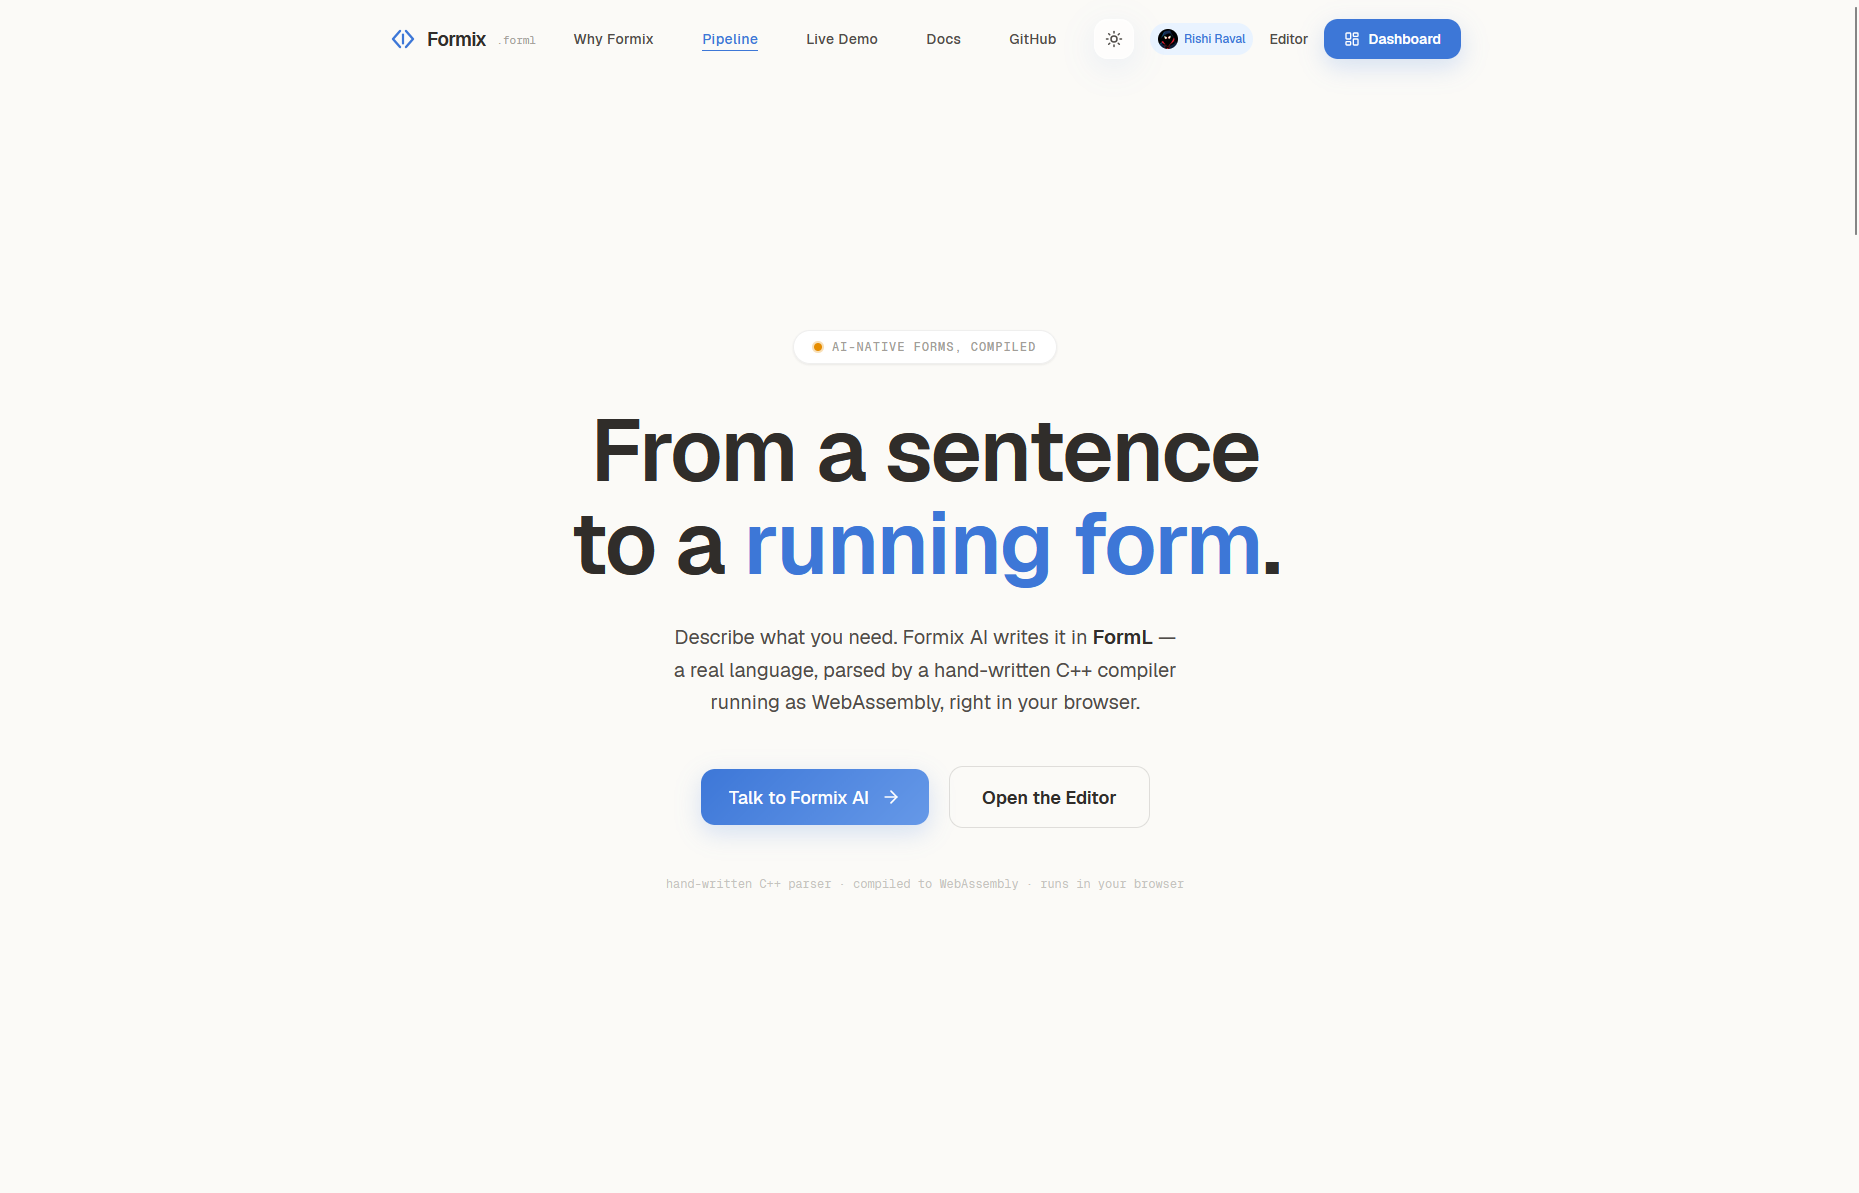
\includegraphics[width=\textwidth]{figures/landing-page.png}
\caption{Formix landing page and product positioning}
\label{fig:landing}
\end{figure}

% =============================================================================
\chapter{System Analysis}
% =============================================================================

\section{Need for the System}
Form definitions frequently outlive the person who created them. A sustainable system must
make the definition readable, reviewable, testable, and portable. A DSL supplies a stable text
representation; a compiler provides early diagnostics; source control records history; and
immutable releases separate experimentation from production. This combination also constrains
generative AI: the model proposes source, while deterministic software decides whether that
source is acceptable.

\section{Preliminary Investigation}
The investigation compared three approaches: building every form directly in React, storing
JSON configuration, and defining a textual DSL. Direct React development gives maximum control
but is too costly for routine forms. JSON is machine-friendly but verbose and has weak
authoring ergonomics. A purpose-built DSL is concise and can express domain constraints, while
its compiler emits JSON for the renderer. The DSL approach was selected because it separates
the authoring representation from the rendering implementation without sacrificing validation.

\section{Actors and Major Use Cases}
\begin{table}[H]
\centering
\caption{Actors and use cases}
\label{tab:actors}
\begin{tabularx}{\textwidth}{>{\bfseries}p{0.22\textwidth}X}
\toprule
Actor & Major use cases\\
\midrule
Project owner & Create projects, invite members, assign roles, configure webhooks, publish and roll back releases\\
Editor & Author FormL, use AI assistance, preview, publish, inspect responses and analytics\\
Viewer & Read project forms and release information without modifying them\\
Respondent & Open public or embedded form, save progress, resume, validate, and submit\\
External system & Receive signed webhook events and verify their HMAC signature\\
CI runner & Compile-check committed FormL fixtures and reject invalid changes\\
\bottomrule
\end{tabularx}
\end{table}

\begin{figure}[H]
\centering
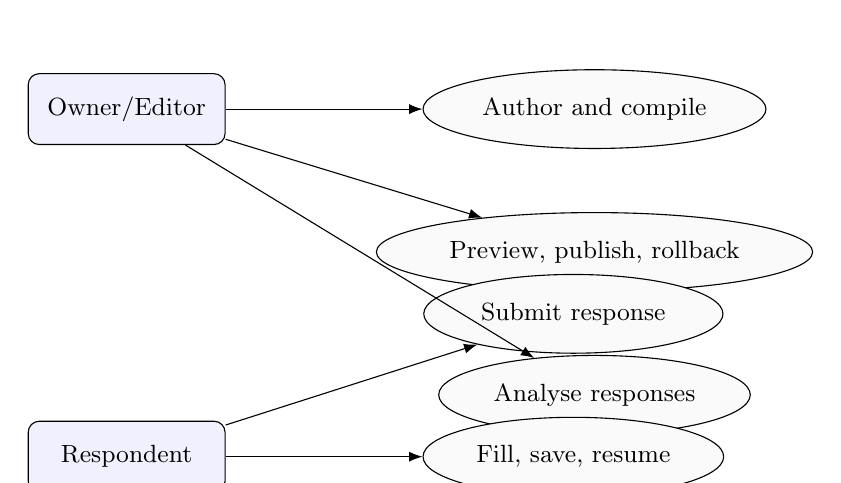
\begin{tikzpicture}[node distance=10mm and 16mm, every node/.style={font=\small},
actor/.style={draw,rounded corners,fill=blue!6,minimum width=25mm,minimum height=9mm},
use/.style={draw,ellipse,fill=black!2,align=center,minimum width=38mm,minimum height=10mm}]
\node[actor] (owner) {Owner/Editor};
\node[actor,below=35mm of owner] (respondent) {Respondent};
\node[use,right=25mm of owner] (author) {Author and compile};
\node[use,below=8mm of author] (release) {Preview, publish, rollback};
\node[use,below=8mm of release] (analyse) {Analyse responses};
\node[use,right=25mm of respondent] (fill) {Fill, save, resume};
\node[use,above=8mm of fill] (submit) {Submit response};
\draw[-{Latex}] (owner) -- (author);
\draw[-{Latex}] (owner) -- (release);
\draw[-{Latex}] (owner) -- (analyse);
\draw[-{Latex}] (respondent) -- (fill);
\draw[-{Latex}] (respondent) -- (submit);
\end{tikzpicture}
\caption{Simplified Formix use-case model}
\label{fig:usecase}
\end{figure}

% =============================================================================
\chapter{Feasibility Study}
% =============================================================================

\section{Technical Feasibility}
The project uses mature open technologies that interoperate over JSON and HTTP. C++20 is
suitable for a deterministic compiler and Emscripten allows the same implementation to run in
the browser. Next.js and React support the editor and public application, while FastAPI and
SQLAlchemy provide typed APIs and portable persistence. The accepted model fits the available
Kaggle training environment by using QLoRA rather than full-parameter fine-tuning.

The main technical risk is the breadth of the system. It is controlled through separation of
responsibilities: the compiler owns language correctness, the frontend owns interaction, and
the backend owns identity and durable state. Immutable release rows avoid copying production
logic into the editor. The webhook subsystem persists a delivery before attempting the network
request, preventing transient failures from silently losing events.

\section{Economic Feasibility}
Development and demonstration can be performed with free or educational tiers: local tooling,
GitHub Actions, Vercel, Render, Neon, and Kaggle. The design avoids a paid parser generator and
does not require a proprietary form SDK. Operating cost will grow with submissions, model
inference, data retention, and webhook traffic, but these costs correspond to product usage and
can be covered by future subscription tiers.

\section{Operational Feasibility}
The graphical preview keeps the DSL approachable for non-compiler specialists. Authors can
write source or ask the assistant, observe diagnostics, and publish only compiler-accepted
output. Respondents use a normal web form and do not need to understand FormL. Preview links,
rollback, audit-friendly releases, and collaborator roles reduce operational risk for teams.

\section{Schedule Feasibility}
The project was divided into language design, compiler implementation, frontend authoring,
backend services, AI evaluation, and product-hardening stages. Each stage produced a runnable
artifact and a verification gate. This incremental arrangement allowed the compiler and
renderer to remain useful even when remote model inference was unavailable.

% =============================================================================
\chapter{Literature Survey}
% =============================================================================

\section{Work by Other Researchers and Existing Systems}
Compiler design separates scanning, parsing, semantic analysis, and code or data generation
into explicit stages \citep{craftinginterpreters,dragonbook}. Domain-specific languages apply
these principles to a restricted problem area, improving expressiveness and validation at the
cost of language maintenance \citep{fowlerdsl}. WebAssembly provides a portable execution
target that enables compiled languages to run in web browsers \citep{webassembly}.

Existing form products demonstrate the value of hosted collection and visual authoring, while
schema-driven libraries demonstrate reusable rendering. However, visual builders often hide
their representation, and generic schemas do not necessarily provide domain-aware compiler
diagnostics. \formix\ combines a compact textual language, a hand-written educational compiler,
and a hosted product workflow.

\section{Benefits Identified from the Survey}
The survey suggested four useful principles. First, syntax and semantics should be distinct so
that diagnostics can state whether a form is malformed or merely inconsistent. Second, the
language should compile to a neutral AST rather than directly manipulating UI components.
Third, browser execution reduces latency and keeps source local during ordinary compilation.
Fourth, generative AI should operate behind deterministic validation and measurable evaluation,
not be treated as a replacement for the compiler.

\section{Proposed Solution}
The proposed system uses \forml\ as the canonical authoring language. The C++ compiler emits a
JSON AST consumed by one shared React renderer. The backend stores projects, sources, compiled
schemas, releases, responses, and integration state. AI generation is an optional authoring
path whose output is compiled and, when necessary, repaired using diagnostic feedback.

\section{Technology Selection}
\begin{table}[H]
\centering
\caption{Technology selection rationale}
\label{tab:tech-selection}
\begin{tabularx}{\textwidth}{>{\bfseries}p{0.18\textwidth}p{0.25\textwidth}X}
\toprule
Concern & Selection & Rationale\\
\midrule
Compiler & C++20 & Explicit ownership, strong types, native speed, and Emscripten support\\
Editor & Monaco & Mature code-editing behaviour, diagnostics, minimap, and keyboard support\\
Web UI & Next.js/React & Component reuse across editor preview, public form, and analytics\\
API & FastAPI & Typed request validation, generated OpenAPI schema, simple Python integration\\
Database & PostgreSQL & Transactions, indexing, row locking, and managed hosting options\\
AI adapter & Qwen2.5-Coder-3B + QLoRA & Code-oriented base model that can be adapted within Kaggle constraints\\
\bottomrule
\end{tabularx}
\end{table}

% =============================================================================
\chapter{Technical Part}
% =============================================================================

\section{Concept of the System}
\formix\ treats a form definition as a program. A source file is tokenised, parsed into an
abstract syntax tree, checked for semantic consistency, serialized as JSON, and rendered as a
user interface. The compiler returns diagnostics rather than throwing on ordinary source
errors, enabling the editor and AI repair loop to show several problems in a single pass.

\begin{figure}[H]
\centering
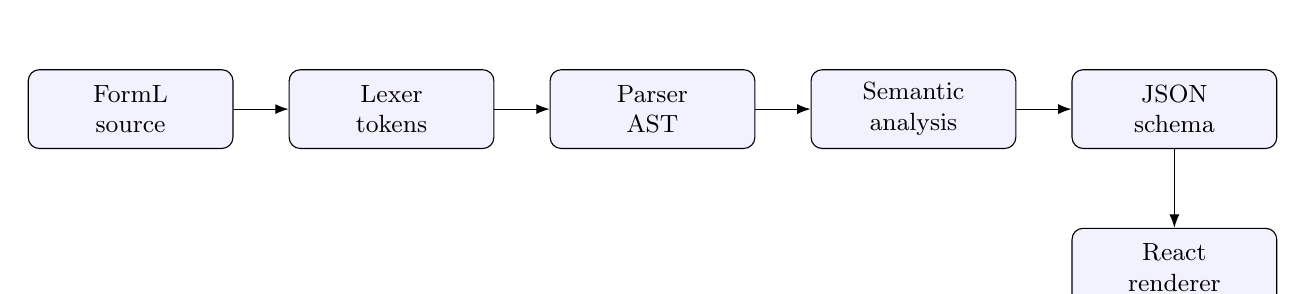
\begin{tikzpicture}[node distance=7mm, every node/.style={font=\small},
stage/.style={draw,rounded corners,minimum width=26mm,minimum height=10mm,align=center,fill=blue!5}]
\node[stage] (source) {FormL\\source};
\node[stage,right=of source] (lexer) {Lexer\\tokens};
\node[stage,right=of lexer] (parser) {Parser\\AST};
\node[stage,right=of parser] (semantic) {Semantic\\analysis};
\node[stage,right=of semantic] (json) {JSON\\schema};
\node[stage,below=10mm of json] (render) {React\\renderer};
\draw[-{Latex}] (source)--(lexer);
\draw[-{Latex}] (lexer)--(parser);
\draw[-{Latex}] (parser)--(semantic);
\draw[-{Latex}] (semantic)--(json);
\draw[-{Latex}] (json)--(render);
\end{tikzpicture}
\caption{FormL compilation and rendering pipeline}
\label{fig:pipeline}
\end{figure}

\section{FormL Language}
The grammar includes primitive typed fields, option fields, UI metadata, validation rules,
pages, sections, rows, columns, reusable groups, variables, conditionals, repeats, computed
fields, URL-backed options, uploads, and actions. The language deliberately uses a small number
of regular constructs so that it remains readable and can be parsed by a hand-written
recursive-descent parser.

\begin{lstlisting}[caption={Representative FormL form},label={lst:forml}]
form "Conference Registration" {
  field full_name: text
    ui { label: "Full name" }
    validate { required minLength: 2 }

  field attendance: radio {
    option "In person"
    option "Online"
  } ui { label: "Attendance mode" }

  field dietary_preferences: checkbox {
    option "Vegetarian"
    option "Vegan"
    option "Gluten-free"
    option "No restrictions"
  } ui { label: "Dietary preferences" }
}
\end{lstlisting}

Dynamic structures are represented directly rather than generated by ad-hoc UI code. For
example, a respondent-controlled repeat count must refer to an integer field, allowing semantic
analysis to reject a fixed variable used where user input is required.

\begin{lstlisting}[caption={Respondent-controlled repeat block},label={lst:repeat}]
form "Book Log" {
  field book_count: integer
    ui { label: "Number of books read" }
    validate { min: 1 max: 20 }

  repeat count = book_count {
    field book_title: text ui { label: "Book title" }
    field release_date: date ui { label: "Release date" }
    field author: text ui { label: "Author" }
  }
}
\end{lstlisting}

\section{Application Areas}
The language and platform can support event registrations, admissions, job applications,
surveys, health check-ins, order requests, lead collection, consent forms, support tickets, and
internal operational workflows. The same source can be reviewed in Git, embedded in a website,
or published through the hosted respondent interface.

\section{Compiler Internals}
The lexer scans source characters while maintaining line and column positions. It emits typed
tokens and reports unrecognised characters through a diagnostic engine. The recursive-descent
parser contains one method per grammar rule and uses synchronisation points to recover after an
error. AST nodes own their children with \texttt{std::unique\_ptr}, which makes tree ownership
explicit. The semantic analyser then detects duplicate names, undefined references, invalid
types, and construct-specific constraints. Finally, the serializer emits the JSON schema used
by the frontend.

The native compiler is the specification authority. The Emscripten bridge exposes the same
entry point to JavaScript, which prevents the editor from implementing a competing parser.
Compiler diagnostics are also supplied to the AI repair prompt, making repair evidence-based
rather than conversational guesswork.

\begin{figure}[H]
\centering
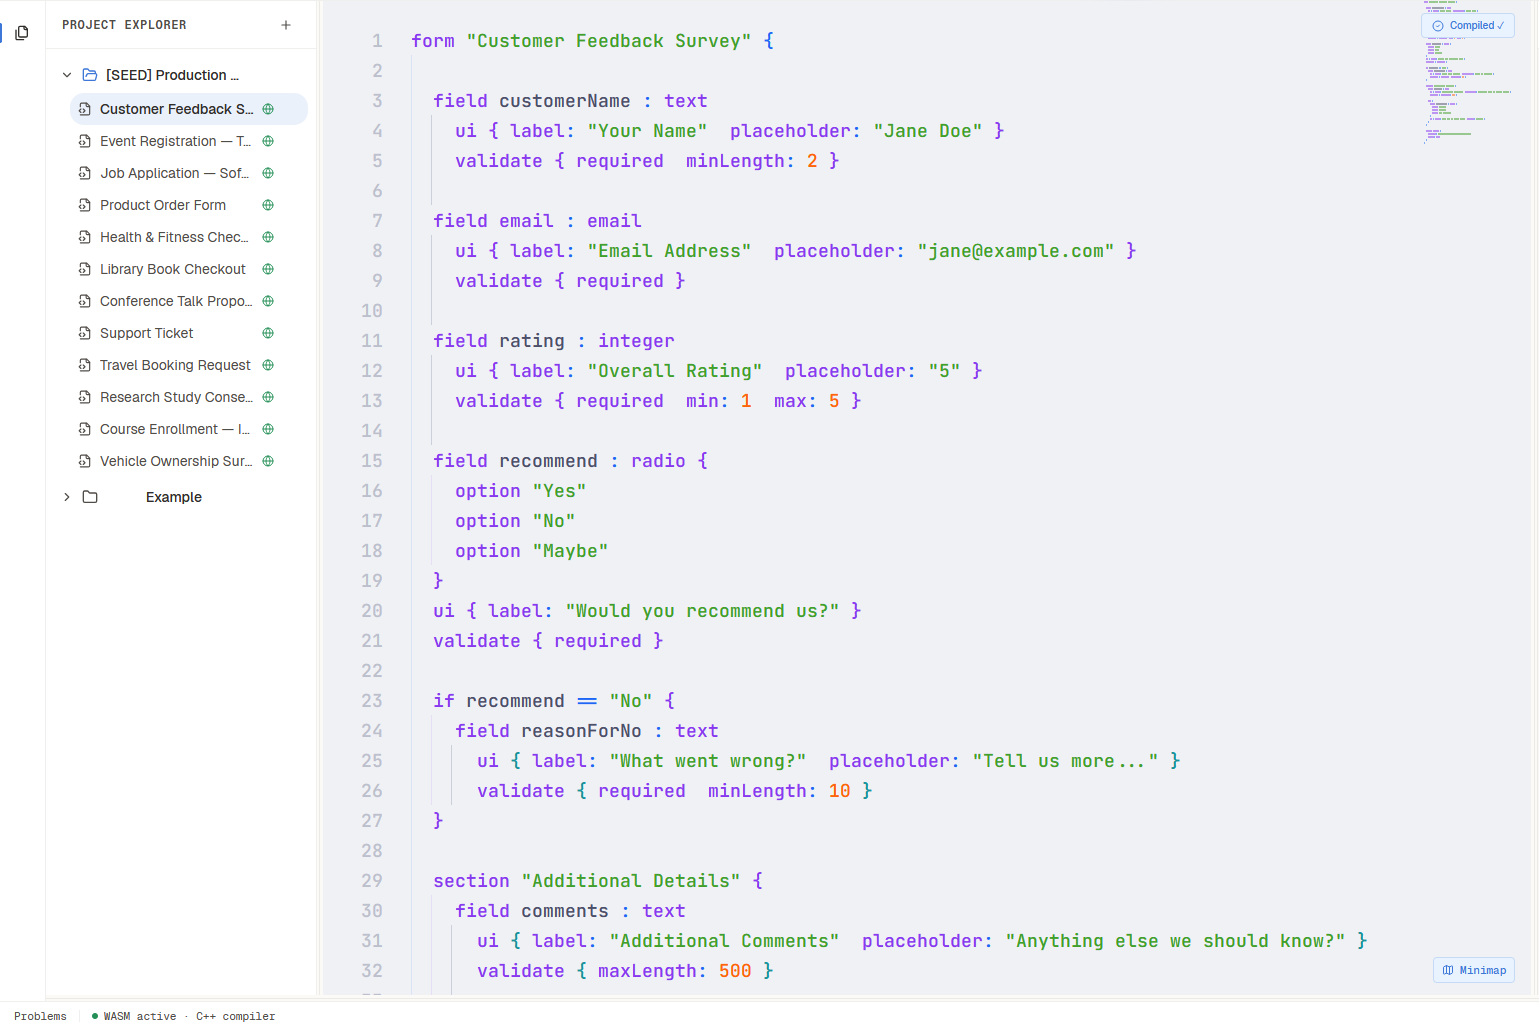
\includegraphics[width=\textwidth]{figures/editor.png}
\caption{Monaco authoring environment with compiler status and project explorer}
\label{fig:editor}
\end{figure}

% =============================================================================
\chapter{Software Engineering Approach}
% =============================================================================

\section{Software Development Paradigm}
\subsection{Description}
An incremental, compiler-first paradigm was used. Language behaviour was expressed through
grammar, fixtures, and diagnostics before higher layers depended on it. The frontend then
consumed the compiler output, followed by persistence, publishing, AI assistance, analytics,
and product-hardening features. Small vertical increments were verified before continuing.

\subsection{Advantages and Disadvantages}
The principal advantage is a stable source of truth: parser and semantic tests reveal language
regressions before they reach users. The approach also supports incremental demonstrations.
Its disadvantage is that changes to the language may require coordinated updates to the
compiler, renderer, documentation, examples, AI dataset, and tests. This cost is controlled by
keeping the AST contract explicit and validating fixtures in CI.

\subsection{Reason for Selection}
The project is both an educational compiler exercise and a real application. A compiler-first
incremental process exposes each language stage for study while avoiding a large, untestable
implementation. It also matches the product requirement that deterministic validation must
remain independent of the AI provider.

\section{Requirement Analysis}
\subsection{Software Requirements Specification}
\begin{longtable}{p{0.12\textwidth}p{0.78\textwidth}}
\caption{Functional requirements}\label{tab:functional}\\
\toprule
\textbf{ID} & \textbf{Requirement}\\
\midrule
\endfirsthead
\toprule
\textbf{ID} & \textbf{Requirement}\\
\midrule
\endhead
FR-01 & The system shall compile FormL and return a JSON AST plus collected diagnostics.\\
FR-02 & The editor shall update the live preview after successful browser-side compilation.\\
FR-03 & Users shall authenticate by local credentials or supported OAuth providers.\\
FR-04 & Owners shall assign editor or viewer roles to existing Formix accounts.\\
FR-05 & Publishing shall create immutable releases in preview or production.\\
FR-06 & An authorised user shall roll an environment back to a prior release.\\
FR-07 & Respondents shall submit public forms and optionally save and resume a draft.\\
FR-08 & Configured webhook events shall be signed, persisted, retried, and replayable.\\
FR-09 & Forms shall be embeddable without installing a framework dependency.\\
FR-10 & AI-generated source shall be compiler checked and repaired within a bounded loop.\\
FR-11 & Dashboards shall display response totals, trends, field summaries, and exports.\\
FR-12 & CI shall reject invalid canonical FormL fixtures and broken production builds.\\
\bottomrule
\end{longtable}

\begin{table}[H]
\centering
\caption{Non-functional requirements}
\label{tab:nonfunctional}
\begin{tabularx}{\textwidth}{>{\bfseries}p{0.22\textwidth}X}
\toprule
Category & Requirement\\
\midrule
Correctness & The compiler is the sole authority for accepted FormL syntax and semantics.\\
Security & Passwords are hashed; access is role checked; webhook payloads are HMAC signed; unsafe literal private webhook destinations are rejected.\\
Reliability & Releases are immutable, submissions retain their release identity, and webhook attempts are stored before transmission.\\
Performance & Ordinary compilation runs locally in WASM; public rendering uses stored compiled JSON.\\
Accessibility & Controls use labels, keyboard-accessible primitives, clear focus states, and reduced-motion-aware UI foundations.\\
Maintainability & Database changes use Alembic; frontend and backend contracts are typed; no parser generator is required.\\
Scalability & Stateless web processes use PostgreSQL; the current polling webhook worker has an explicit migration path to a managed queue.\\
\bottomrule
\end{tabularx}
\end{table}

\subsection{Glossary and Supplementary Specification}
A \emph{draft} is mutable authoring state. A \emph{release} is an immutable snapshot of source
and compiled schema. An \emph{environment} is a movable pointer to a release, currently preview
or production. A \emph{submission} is respondent data pinned to the production release that
accepted it. A \emph{delivery} is one persisted webhook transmission attempt record.

\subsection{Activity and Sequence Models}
\begin{figure}[H]
\centering
\begin{tikzpicture}[node distance=7mm, every node/.style={font=\small},
step/.style={draw,rounded corners,fill=black!2,minimum width=43mm,minimum height=8mm,align=center},
decision/.style={draw,diamond,aspect=2.1,fill=orange!7,align=center}]
\node[step] (prompt) {Enter prompt or edit source};
\node[step,below=of prompt] (generate) {Generate candidate FormL};
\node[step,below=of generate] (compile) {Compile with FormL compiler};
\node[decision,below=9mm of compile] (valid) {Valid?};
\node[step,below left=9mm and 14mm of valid] (repair) {Return diagnostics to repair loop};
\node[step,below right=9mm and 14mm of valid] (preview) {Render verified preview};
\draw[-{Latex}] (prompt)--(generate);
\draw[-{Latex}] (generate)--(compile);
\draw[-{Latex}] (compile)--(valid);
\draw[-{Latex}] (valid)--node[left]{no}(repair);
\draw[-{Latex}] (repair.west) -| ++(-12mm,0) |- (compile.west);
\draw[-{Latex}] (valid)--node[right]{yes}(preview);
\end{tikzpicture}
\caption{Compiler-guided AI generation activity}
\label{fig:ai-activity}
\end{figure}

\begin{figure}[H]
\centering
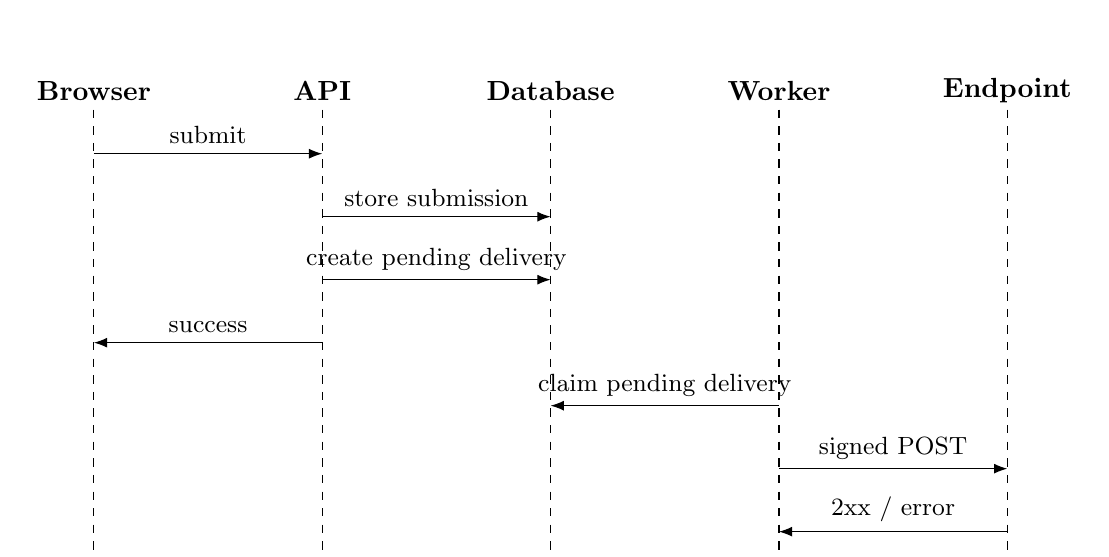
\begin{tikzpicture}[x=1.45cm,y=0.8cm,>=Latex,font=\small]
\foreach \x/\name in {0/Browser,2/API,4/Database,6/Worker,8/Endpoint}{
  \node[font=\bfseries] at (\x,0) {\name};
  \draw[dashed] (\x,-0.3)--(\x,-7.6);
}
\draw[->] (0,-1)--node[above]{submit} (2,-1);
\draw[->] (2,-2)--node[above]{store submission} (4,-2);
\draw[->] (2,-3)--node[above]{create pending delivery} (4,-3);
\draw[->] (2,-4)--node[above]{success} (0,-4);
\draw[->] (6,-5)--node[above]{claim pending delivery} (4,-5);
\draw[->] (6,-6)--node[above]{signed POST} (8,-6);
\draw[->] (8,-7)--node[above]{2xx / error} (6,-7);
\end{tikzpicture}
\caption{Submission and durable webhook sequence}
\label{fig:webhook-sequence}
\end{figure}

\section{Planning and Managerial Aspects}
\subsection{Project Scope and Resources}
The work was completed by one student using a Windows development machine, GitHub source
control, free hosted services, Kaggle GPU notebooks, and open-source frameworks. The repository
and compiler fixtures are the primary configuration records.

\subsection{Schedule and Estimation}
\begin{table}[H]
\centering
\caption{Indicative project schedule}
\label{tab:schedule}
\begin{tabularx}{\textwidth}{>{\bfseries}p{0.16\textwidth}X p{0.18\textwidth}}
\toprule
Phase & Deliverable & Relative effort\\
\midrule
1 & Requirements, FormL grammar, compiler plan & Medium\\
2 & Lexer, AST, parser, semantic analysis, serialization & High\\
3 & WASM bridge, editor, renderer, diagnostics & High\\
4 & Authentication, projects, persistence, publishing & High\\
5 & AI data, QLoRA training, evaluation and repair loop & High\\
6 & Analytics, collaboration, releases, webhooks, embed, drafts & High\\
7 & Verification, deployment documentation, report & Medium\\
\bottomrule
\end{tabularx}
\end{table}

\subsection{Risk Analysis}
\begin{table}[H]
\centering
\caption{Major risks and mitigations}
\label{tab:risks}
\begin{tabularx}{\textwidth}{p{0.27\textwidth}p{0.18\textwidth}X}
\toprule
Risk & Impact & Mitigation\\
\midrule
AI produces plausible invalid syntax & High & Compiler judge, bounded repair loop, held-out evaluation\\
Language and renderer diverge & High & Shared AST contract and canonical fixtures\\
Production overwritten by preview & High & Immutable releases and separate environment pointers\\
Webhook outage loses an event & High & Persist-before-send, exponential retry, logs and replay\\
Unauthorised project modification & High & Central owner/editor/viewer checks\\
Schema migration breaks deployment & High & Additive Alembic migration tested on a fresh database\\
Free-tier inference unavailable & Medium & Provider fallback and compiler/editor remain independently usable\\
\bottomrule
\end{tabularx}
\end{table}

\subsection{Security and Configuration Management}
Authentication uses signed JWT sessions and hashed passwords, with OAuth account linking for
Google and GitHub. Project access is centralised by role. Resume tokens and preview tokens are
high-entropy values, and webhook secrets are shown once. Delivery signatures use HMAC-SHA256.
Secrets are supplied through environment variables and are not committed. Alembic controls
database schema versions; Git records source and report history; CI verifies proposed changes.

\section{Design}
\subsection{Architectural Design}
\begin{figure}[H]
\centering
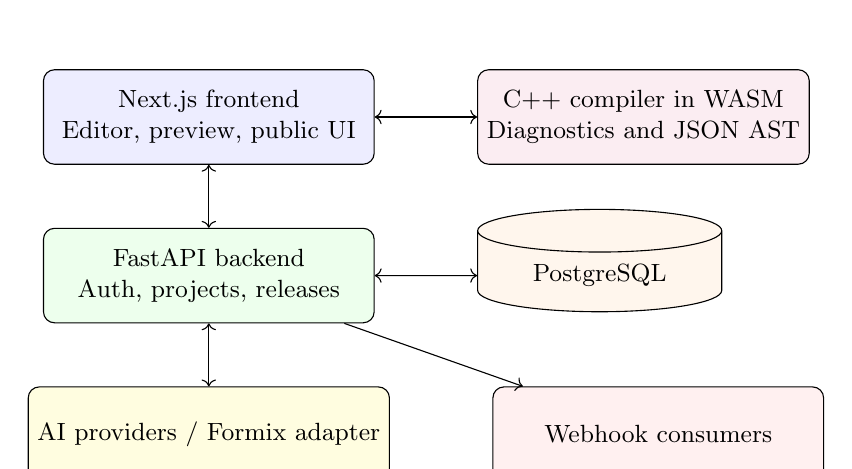
\begin{tikzpicture}[node distance=8mm and 13mm,font=\small,
box/.style={draw,rounded corners,minimum width=42mm,minimum height=12mm,align=center},
store/.style={draw,cylinder,shape border rotate=90,aspect=0.28,minimum width=31mm,minimum height=13mm,align=center}]
\node[box,fill=blue!7] (front) {Next.js frontend\\Editor, preview, public UI};
\node[box,fill=purple!7,right=of front] (wasm) {C++ compiler in WASM\\Diagnostics and JSON AST};
\node[box,fill=green!7,below=of front] (api) {FastAPI backend\\Auth, projects, releases};
\node[store,fill=orange!7,right=of api] (db) {PostgreSQL};
\node[box,fill=yellow!12,below=of api] (ai) {AI providers / Formix adapter};
\node[box,fill=red!6,right=of ai] (external) {Webhook consumers};
\draw[<->] (front)--(wasm);
\draw[<->] (front)--(api);
\draw[<->] (api)--(db);
\draw[<->] (api)--(ai);
\draw[->] (api)--(external);
\end{tikzpicture}
\caption{High-level Formix architecture}
\label{fig:architecture}
\end{figure}

The frontend and backend are deployable independently. Compiler execution remains local to the
browser for authoring, while the backend stores the compiled schema used by public pages. A
release row snapshots both source and schema. Production and preview fields on the form point to
specific releases, enabling constant-time rollback without rewriting history.

\subsection{Data Model}
\begin{table}[H]
\centering
\caption{Principal persistent entities}
\label{tab:data-model}
\begin{tabularx}{\textwidth}{>{\bfseries}p{0.22\textwidth}X}
\toprule
Entity & Responsibility\\
\midrule
User & Identity, credentials, OAuth links, profile\\
Project / ProjectMember & Form grouping, ownership, editor/viewer membership\\
Form & Mutable source and active preview/production release pointers\\
FormRelease & Immutable versioned source and compiled schema\\
Submission & Response data, completion metadata, associated release\\
FormDraft & Anonymous resumable response with expiry and token\\
WebhookEndpoint & Configured URL, subscribed events, signing secret, status\\
WebhookDelivery & Payload, attempts, response status, next retry and error\\
\bottomrule
\end{tabularx}
\end{table}

\subsection{Interface Design}
The editor uses a restrained three-pane layout: project explorer, Monaco source editor/live
preview, and AI assistant. Release, collaboration, and integration controls are kept in focused
dialogs so that the primary authoring path remains uncluttered. The same renderer powers editor
preview and public forms, reducing visual divergence.

\begin{figure}[H]
\centering
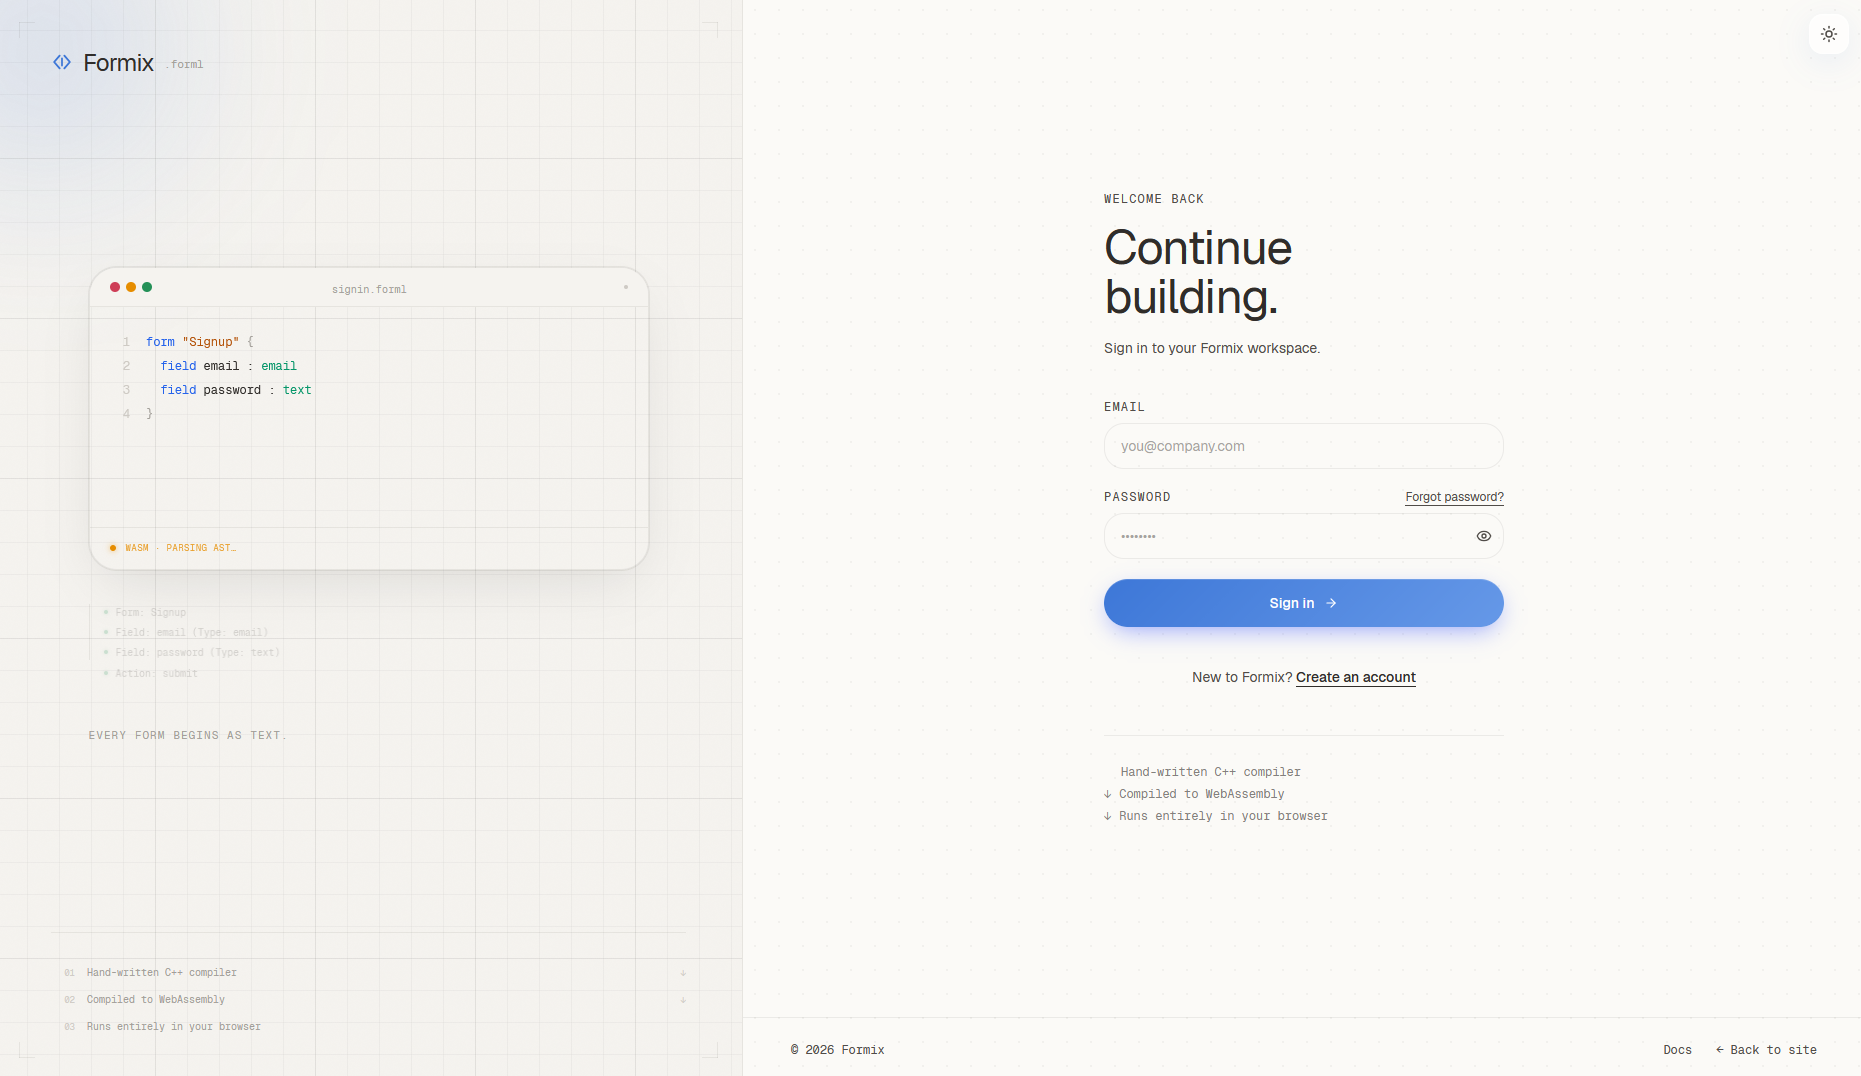
\includegraphics[width=0.78\textwidth]{figures/sign-in.png}
\caption{Formix sign-in interface}
\label{fig:signin}
\end{figure}

\section{Implementation}
\subsection{Language and Coding Characteristics}
C++ compiler code uses value types and \texttt{std::unique\_ptr} ownership; user source errors
are collected as diagnostics rather than exceptions. TypeScript supplies frontend contracts and
Python type models validate API boundaries. The implementation reuses shared access and renderer
functions instead of duplicating checks in individual routes.

\subsection{Release Management}
Publishing locks the form row, increments a release counter, and inserts a snapshot. A preview
publish updates only the preview pointer; production remains unchanged. Rollback changes the
selected environment pointer to an earlier compatible release. Submissions record the active
production release, preserving the historical meaning of response data.

\subsection{Reliable Integrations}
Configured webhooks are stored per form. On submission, a delivery row is inserted before any
network call. The worker signs the raw payload, sends it, stores the result, and schedules an
exponential retry after failure. An authorised editor can inspect delivery history and replay a
failed event. The current database-polling worker is intentionally simple and suitable for the
minor-project scale; a managed queue is the documented upgrade when concurrent delivery volume
outgrows it.

\subsection{Save-and-Resume and Embedding}
Anonymous drafts use opaque tokens and expire after 30 days. The public form saves after a short
debounce, updates the URL with the token, and deletes the draft after successful submission.
The dependency-free embed script discovers elements carrying a form identifier, creates a
sandboxed iframe, and adjusts height from validated messages sent by the public renderer.

\subsection{AI-Assisted Form Generation}
The backend supports an OpenAI-compatible fine-tuned endpoint and a provider fallback chain.
The accepted demonstration adapter is a rank-32 QLoRA adaptation of
\texttt{Qwen/Qwen2.5-Coder-3B-Instruct}. Training and evaluation run on Kaggle, while deployment
remains optional. Candidate source is extracted, compiled, and repaired at most a bounded number
of times using exact diagnostics.

\begin{table}[H]
\centering
\caption{Accepted fine-tuned model evaluation on 132 held-out examples}
\label{tab:model-results}
\begin{tabular}{lr}
\toprule
Metric & Result\\
\midrule
First-pass compile rate & 96.97\%\\
Compile rate after repair & 97.73\%\\
Mean field coverage & 99.62\%\\
Mean field precision & 99.62\%\\
Exact field-set rate & 99.24\%\\
Required-pattern coverage & 96.21\%\\
Intent success rate & 95.45\%\\
Unchanged-edit rate & 0.00\%\\
\bottomrule
\end{tabular}
\end{table}

\begin{figure}[H]
\centering
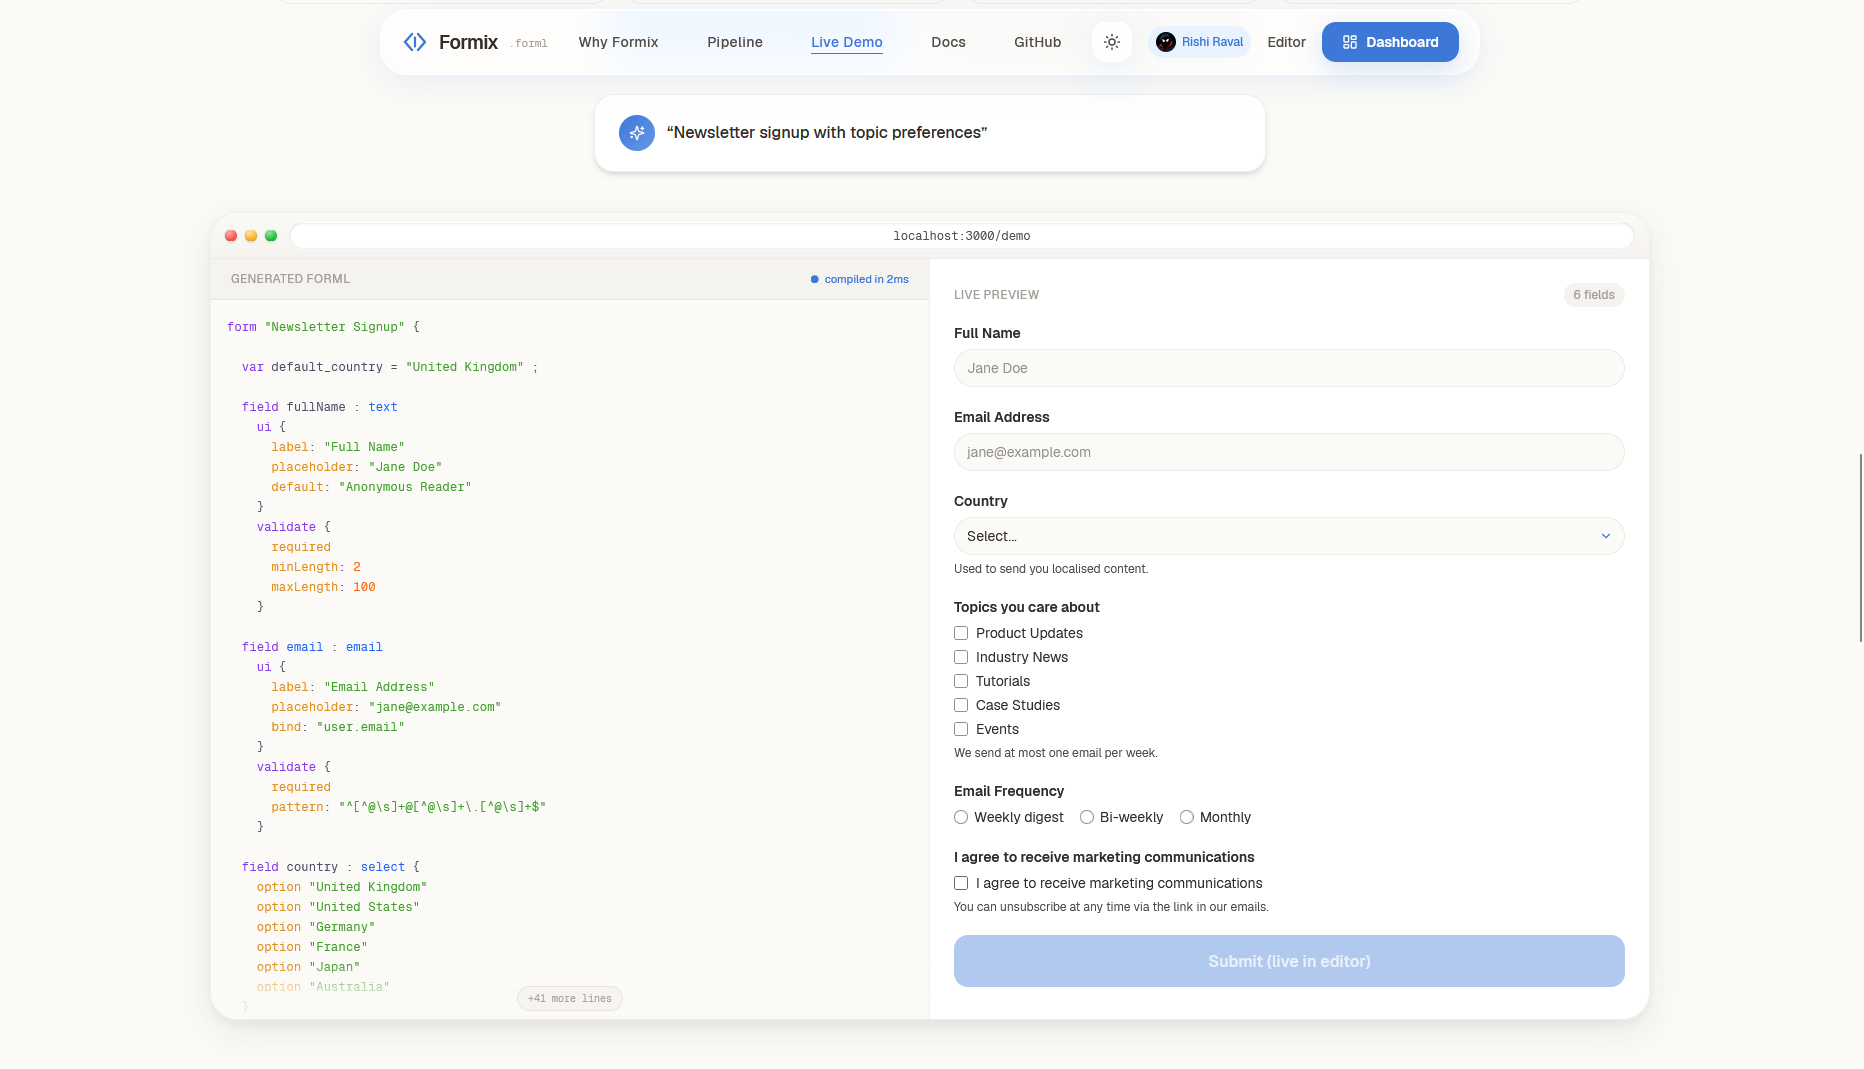
\includegraphics[width=0.93\textwidth]{figures/live-demo.png}
\caption{Live demonstration of generated FormL and its rendered result}
\label{fig:demo}
\end{figure}

\subsection{Continuous Integration}
The repository includes a no-dependency validation script that loads the production WASM
compiler and checks supplied \texttt{.forml} files. GitHub Actions installs exact frontend
dependencies, runs tests, creates a production build, and validates a canonical compiler fixture.
This gives language changes a small executable check without introducing another framework.

\section{Testing}
\subsection{Objectives and Strategy}
Testing targets the boundaries where one subsystem trusts another: FormL to AST, source to
renderer, user to project, draft token to data, release to production, and submission to webhook.
The strategy combines compiler fixtures, TypeScript unit tests, direct backend route/database
checks, migration tests, model evaluation, and a complete production frontend build.

\begin{table}[H]
\centering
\caption{Verification summary}
\label{tab:verification}
\begin{tabularx}{\textwidth}{>{\bfseries}p{0.26\textwidth}p{0.19\textwidth}X}
\toprule
Check & Result & Coverage\\
\midrule
Frontend automated tests & 34 passed & FormL helpers, AI loop, renderer utilities and regressions\\
Startup-platform backend checks & 4 passed & Releases/rollback, drafts, RBAC, webhook safety/secret handling\\
Alembic migration & Passed & Fresh database upgraded through the new head revision\\
Production build & Passed & Next.js route compilation including public and preview form pages\\
WASM FormL validation & Passed & Canonical book-catalog fixture compiled using production assets\\
Fine-tuned evaluation & Quality gate passed & 132 held-out generate/edit/repair examples\\
\bottomrule
\end{tabularx}
\end{table}

\subsection{Representative Test Data}
Test forms include contact forms, conference registrations with dietary preferences, dynamic
book/dependent repeats, conditional guardian fields, multi-page job applications, computed
orders, uploads, and URL-backed select options. Negative fixtures exercise missing delimiters,
invalid block syntax, undefined references, unsupported upload accept values, and malformed
computed expressions.

\begin{figure}[H]
\centering
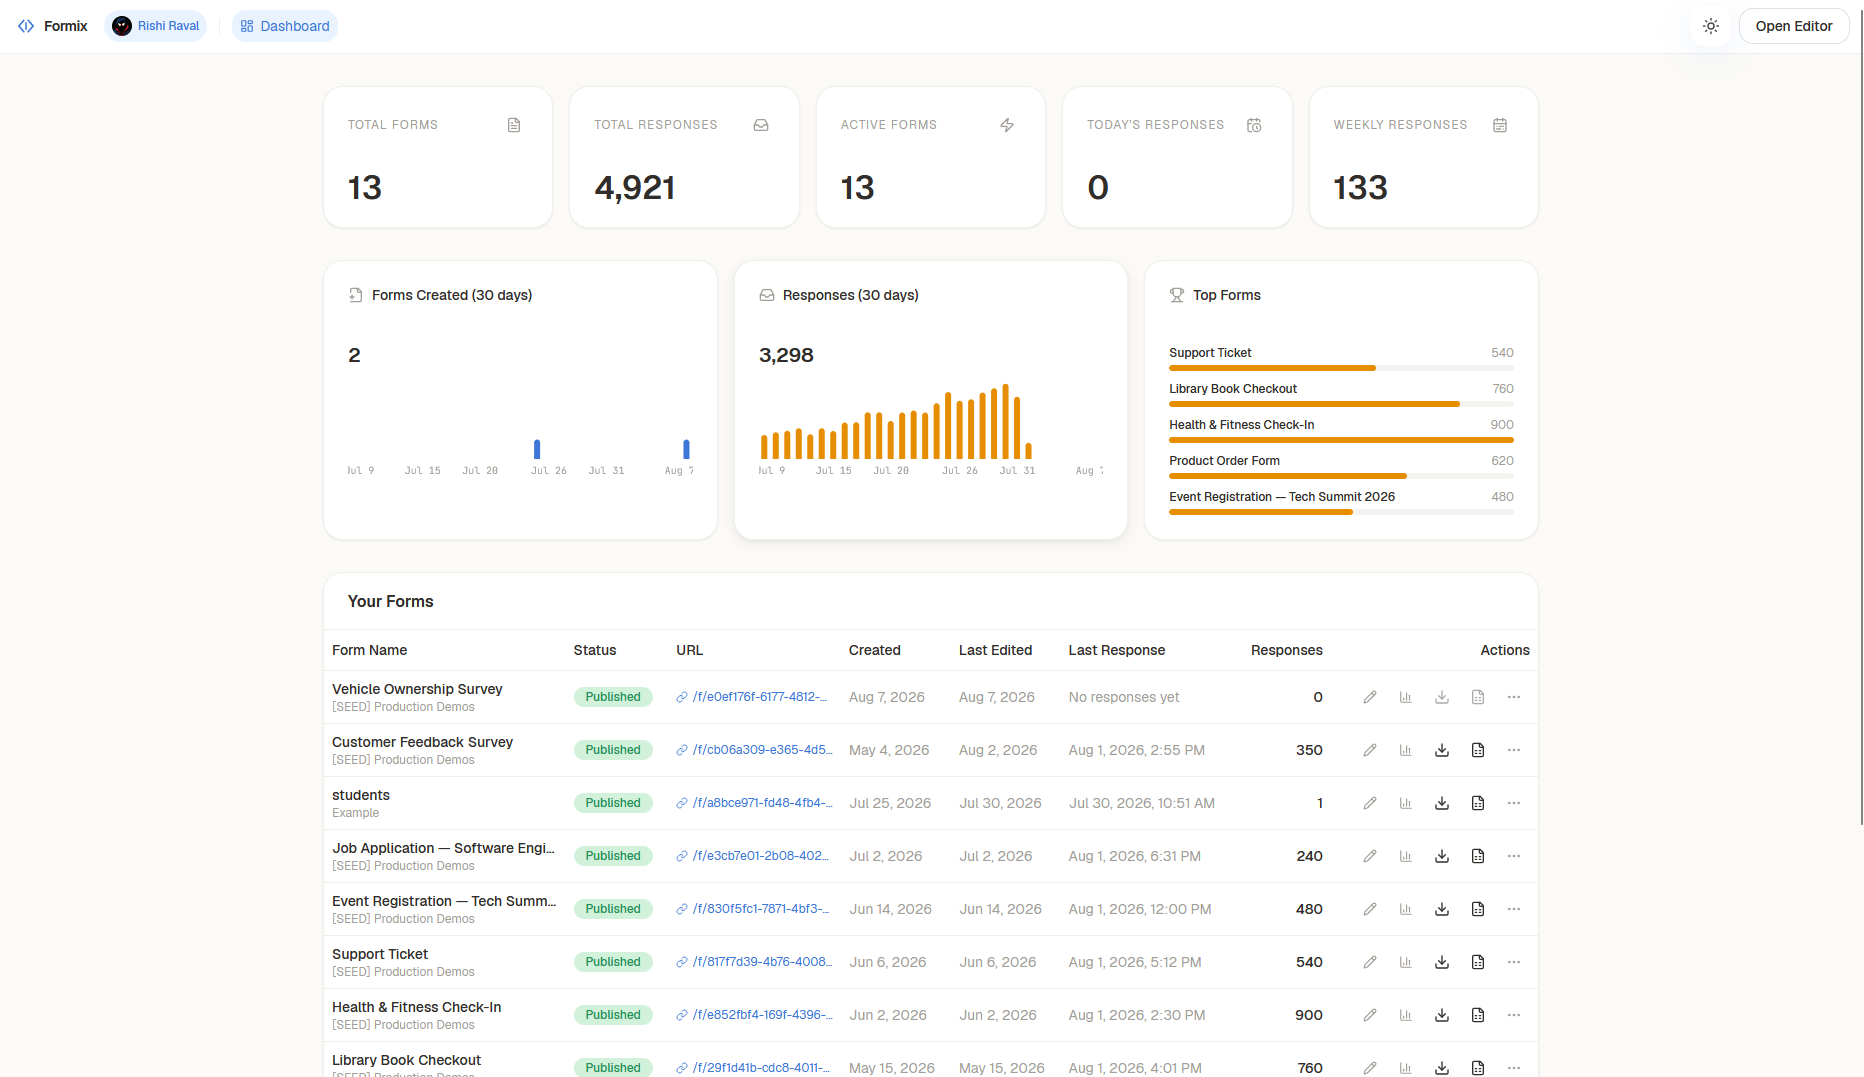
\includegraphics[width=\textwidth]{figures/dashboard.png}
\caption{Dashboard showing published forms and aggregate response activity}
\label{fig:dashboard}
\end{figure}

\begin{figure}[H]
\centering
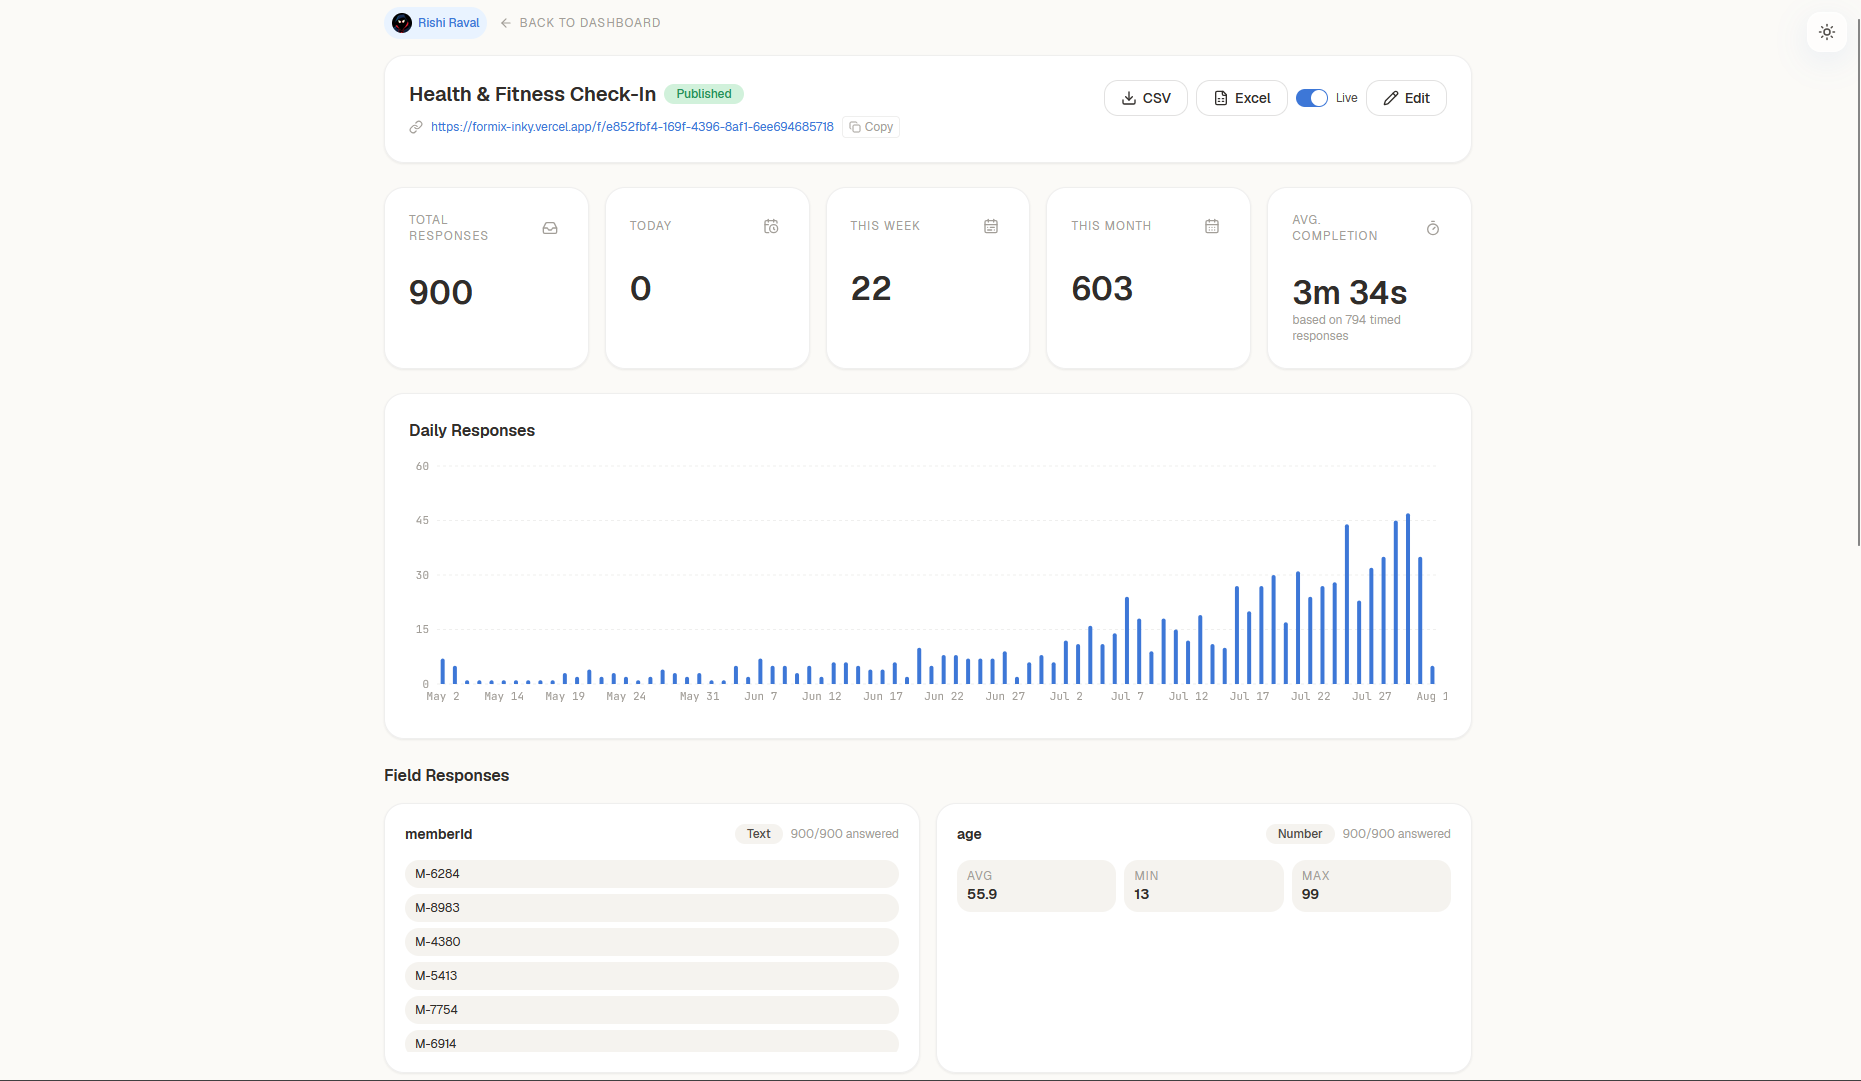
\includegraphics[width=\textwidth]{figures/analytics.png}
\caption{Per-form response analytics and export controls}
\label{fig:analytics}
\end{figure}

% =============================================================================
\chapter{Conclusion and Discussion}
% =============================================================================

\section{Conclusion}
\formix\ demonstrates a complete compiler-driven alternative to opaque form configuration.
The project connects language design, a hand-written C++ compiler, WebAssembly, a modern web
editor, authenticated backend services, public delivery, analytics, and compiler-guided
generative AI. The additional product layer---collaboration roles, immutable environments,
rollback, signed durable webhooks, resumable drafts, an embed SDK, and CI validation---moves the
system from a single-user demonstration toward a scalable software product.

The central architectural result is that the compiler remains the authority. A model may
accelerate authoring, but cannot redefine correctness; the preview cannot overwrite production;
and an integration failure does not erase its own evidence. These properties are more important
for long-term reliability than adding many disconnected visual controls.

\section{Limitations}
The webhook worker currently polls the relational database and should move to a managed queue
for high concurrency. Webhook URL screening blocks literal private addresses but production
hardening should also resolve and re-check DNS targets to resist rebinding. Collaborative
editing is role-based rather than simultaneous CRDT editing. Drafts are anonymous tokens rather
than user-synchronised cross-device records. The AI evaluation set is project-specific and
larger external validation would strengthen generalisation claims. Accessibility has been
considered in components but requires a formal WCAG audit with assistive technologies.

\section{Difficulties Encountered}
The most difficult area was the boundary between valid-looking generated text and valid FormL.
Early model outputs invented array syntax for uploads, block syntax for computed values, and
unsupported tokens such as \texttt{then}. Compiler diagnostics and targeted grammar examples
improved this substantially. Another difficulty was preserving the deployment while extending
the data model; additive migrations and release indirection reduced that risk. Finally, keeping
compiler, renderer, documentation, training examples, and screenshots consistent required
explicit source-of-truth decisions rather than manual duplication.

\section{Future Enhancement}
Future work should prioritise operational foundations over grammar expansion for its own sake:
managed background jobs, delivery observability, billing and quotas, organisation workspaces,
audit logs, regional storage policies, custom domains, template discovery, and end-to-end
accessibility testing. Language evolution can then add carefully specified constructs backed by
grammar, AST, semantic, renderer, documentation, dataset, and fixture updates in one change.
The model evaluation suite should grow with real anonymised failure cases and report results per
scenario, not only aggregate rates.

% =============================================================================
\chapter{Bibliography and References}
% =============================================================================
\renewcommand{\bibname}{References}
\renewcommand{\bibsection}{}
\bibliographystyle{plainnat}
\bibliography{references}

% =============================================================================
\appendix
\chapter{Annexures}
% =============================================================================

\section{Selected Product Screens}
\begin{figure}[H]
\centering
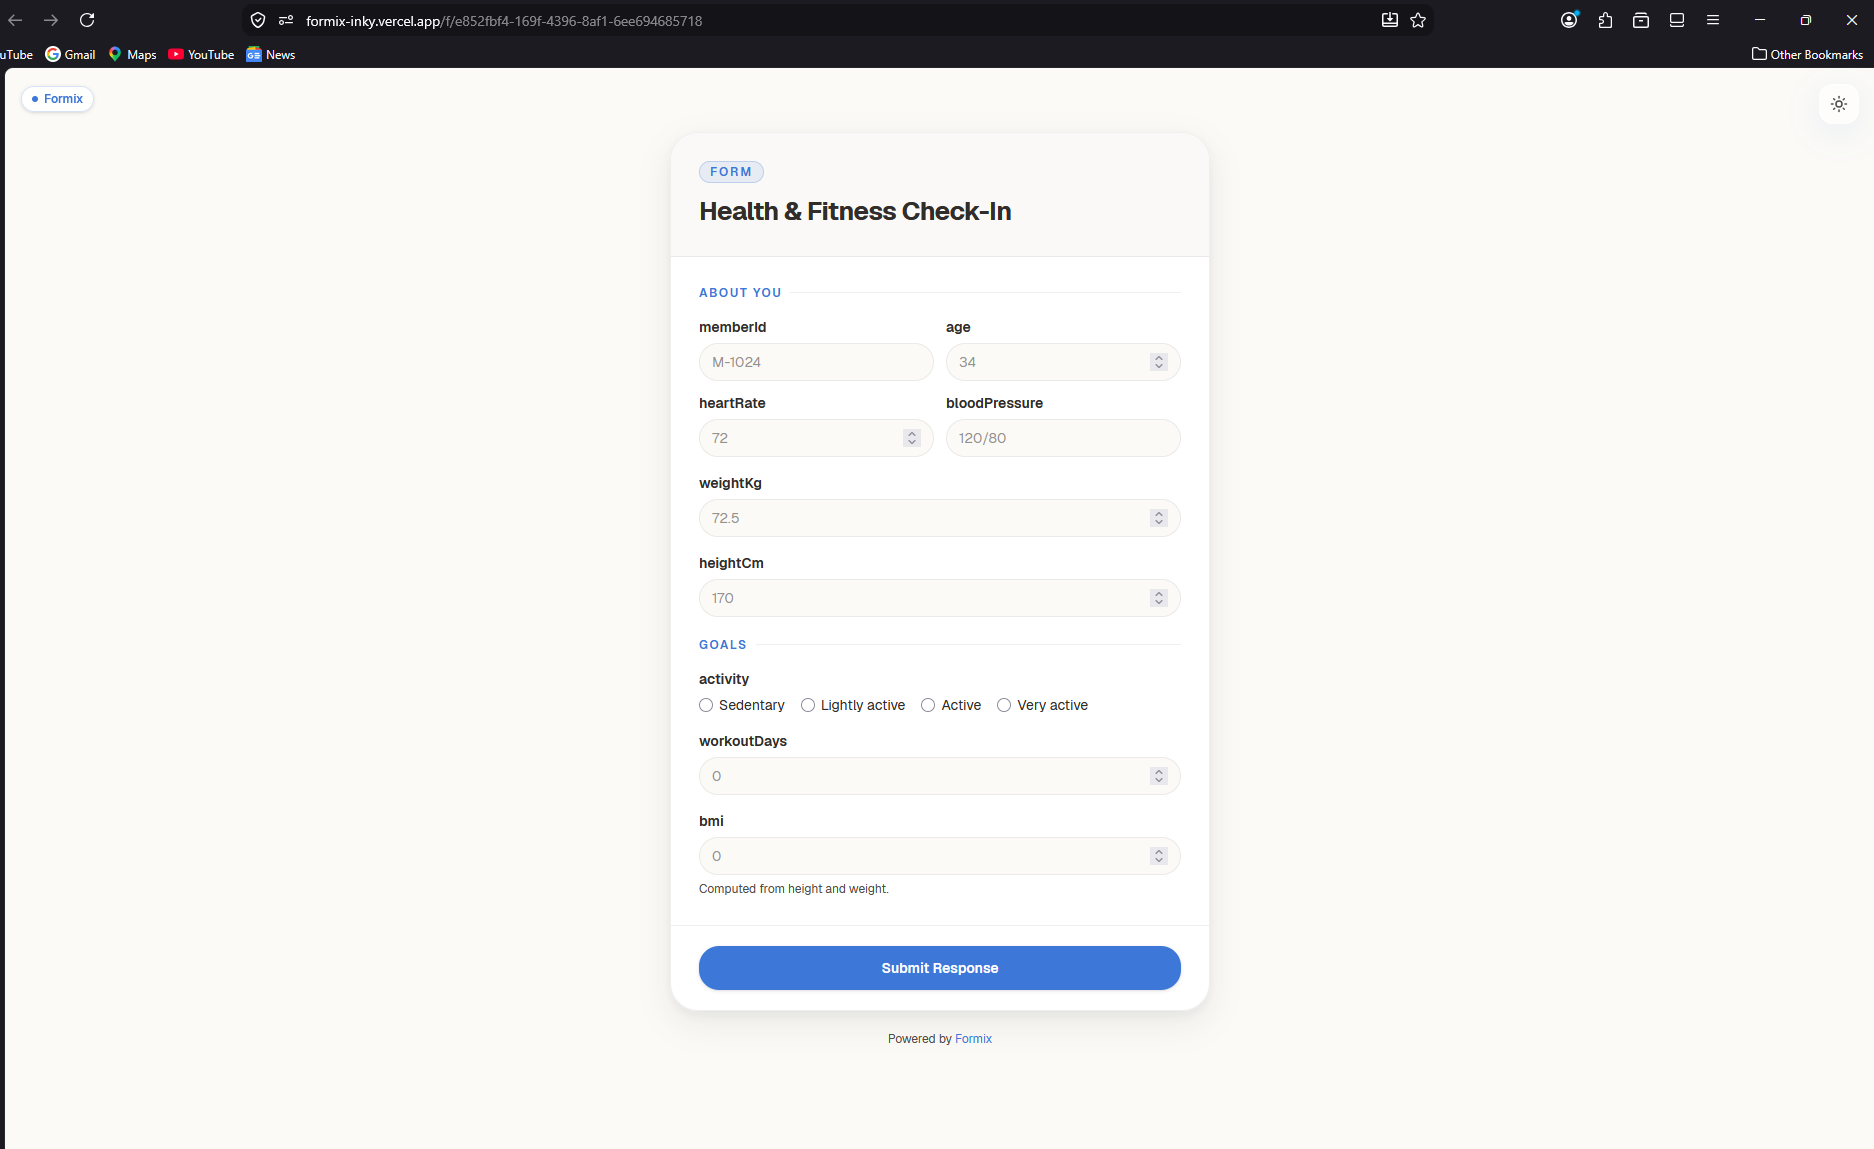
\includegraphics[width=0.72\textwidth]{figures/published-form.png}
\caption{Published respondent form}
\label{fig:published}
\end{figure}

\begin{figure}[H]
\centering
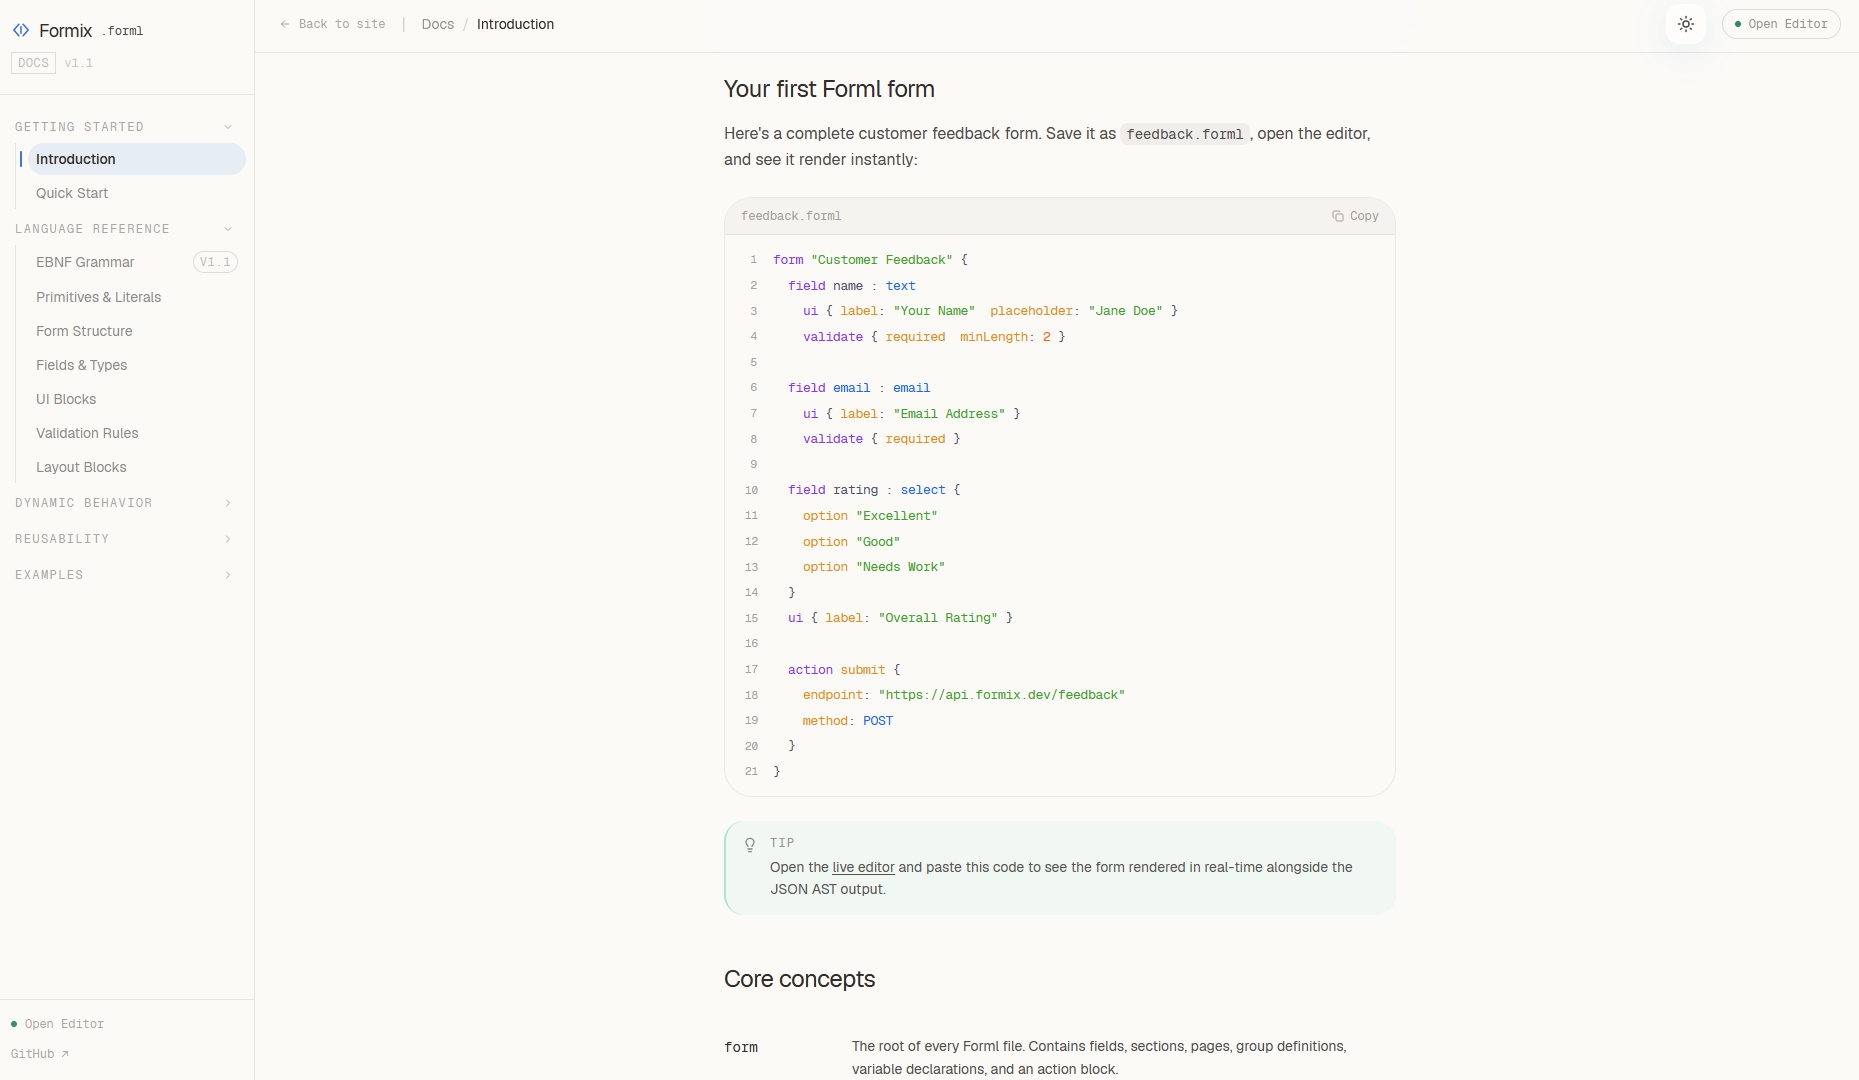
\includegraphics[width=\textwidth]{figures/documentation.png}
\caption{FormL documentation interface}
\label{fig:documentation}
\end{figure}

\section{Deployment Checklist}
\begin{enumerate}
  \item Configure the backend database, JWT secret, allowed origins, OAuth credentials, and optional model endpoint.
  \item Run \texttt{alembic upgrade head} before starting the updated backend.
  \item Build the frontend with \texttt{npm run build} and set \texttt{NEXT\_PUBLIC\_API\_URL} to the backend origin.
  \item Confirm the backend health endpoint, sign-in flow, editor compilation, preview release, production release, public submission, draft resume, and webhook delivery.
  \item Keep the accepted model adapter outside normal Git history because its compressed artifact exceeds the standard per-file GitHub limit.
\end{enumerate}

\section{Compiler Verification Command}
The same production WebAssembly compiler can validate one file or an entire directory:
\begin{lstlisting}[language={},caption={CI-friendly FormL verification}]
npm run forml:check -- path/to/form.forml
\end{lstlisting}

\section{Sample Embed}
\begin{lstlisting}[language=HTML,caption={Dependency-free Formix embed}]
<div data-formix-form="FORM_ID"></div>
<script async src="https://YOUR-FORMIX-DOMAIN/formix-embed.js"></script>
\end{lstlisting}

\end{document}
